\documentclass[aspectratio=169]{../latex_main/tntbeamer}  % you can pass all options of the beamer class, e.g., 'handout' or 'aspectratio=43'
\usepackage{dsfont}
\usepackage{bm}
\usepackage[english]{babel}
\usepackage[T1]{fontenc}
%\usepackage[utf8]{inputenc}
\usepackage{graphicx}
\graphicspath{ {./figures/} }
\usepackage{algorithm}
\usepackage[ruled,vlined,algo2e,linesnumbered]{algorithm2e}
\usepackage{hyperref}
\usepackage{booktabs}
\usepackage{mathtools}

\usepackage{amsmath,amssymb}

\DeclareMathOperator*{\argmax}{arg\,max}
\DeclareMathOperator*{\argmin}{arg\,min}

\usepackage{pgfplots}
\pgfplotsset{compat=1.16}
\usepackage{tikz}
\usetikzlibrary{trees} 
\usetikzlibrary{shapes.geometric}
\usetikzlibrary{positioning,shapes,shadows,arrows,calc,mindmap}
\usetikzlibrary{positioning,fadings,through}
\usetikzlibrary{decorations.pathreplacing}
\usetikzlibrary{intersections}
\pgfdeclarelayer{background}
\pgfdeclarelayer{foreground}
\pgfsetlayers{background,main,foreground}
\tikzstyle{activity}=[rectangle, draw=black, rounded corners, text centered, text width=8em]
\tikzstyle{data}=[rectangle, draw=black, text centered, text width=8em]
\tikzstyle{myarrow}=[->, thick, draw=black]

% Define the layers to draw the diagram
\pgfdeclarelayer{background}
\pgfdeclarelayer{foreground}
\pgfsetlayers{background,main,foreground}

% Requires XeLaTeX or LuaLaTeX
\usepackage{unicode-math}

\usepackage{fontspec}
%\setsansfont{Arial}
\setsansfont{RotisSansSerifStd}[ 
Path=../latex_main/fonts/,
Extension = .otf,
UprightFont = *-Regular,  % or *-Light
BoldFont = *-ExtraBold,  % or *-Bold
ItalicFont = *-Italic
]
\setmonofont{Cascadia Mono}[
Scale=0.8
]

% scale factor adapted; mathrm font added (Benjamin Spitschan @TNT, 2021-06-01)
%\setmathfont[Scale=1.05]{Libertinus Math}
%\setmathrm[Scale=1.05]{Libertinus Math}

% other available math fonts are (not exhaustive)
% Latin Modern Math
% XITS Math
% Libertinus Math
% Asana Math
% Fira Math
% TeX Gyre Pagella Math
% TeX Gyre Bonum Math
% TeX Gyre Schola Math
% TeX Gyre Termes Math

% Literature References
\newcommand{\lit}[2]{\href{#2}{\footnotesize\color{black!60}[#1]}}

%%% Beamer Customization
%----------------------------------------------------------------------
% (Don't) Show sections in frame header. Options: 'sections', 'sections light', empty
\setbeamertemplate{headline}{empty}

% Add header logo for normal frames
\setheaderimage{
	% 
\includegraphics[height=\logoheight]{figures/TNT_darkv4.pdf}
	
\includegraphics[height=\logoheight]{../latex_main/figures/luh_logo_rgb_0_80_155.pdf}
	% 
\includegraphics[height=\logoheight]{figures/logo_tntluh.pdf}
}

% Header logo for title page
\settitleheaderimage{
	% 
\includegraphics[height=\logoheight]{figures/TNT_darkv4.pdf}
	
\includegraphics[height=\logoheight]{../latex_main/figures/luh_logo_rgb_0_80_155.pdf}
	% 
\includegraphics[height=\logoheight]{figures/logo_tntluh.pdf}
}

% Title page: tntdefault 
\setbeamertemplate{title page}[tntdefault]  % or luhstyle
% Add optional title image here
%\addtitlepageimagedefault{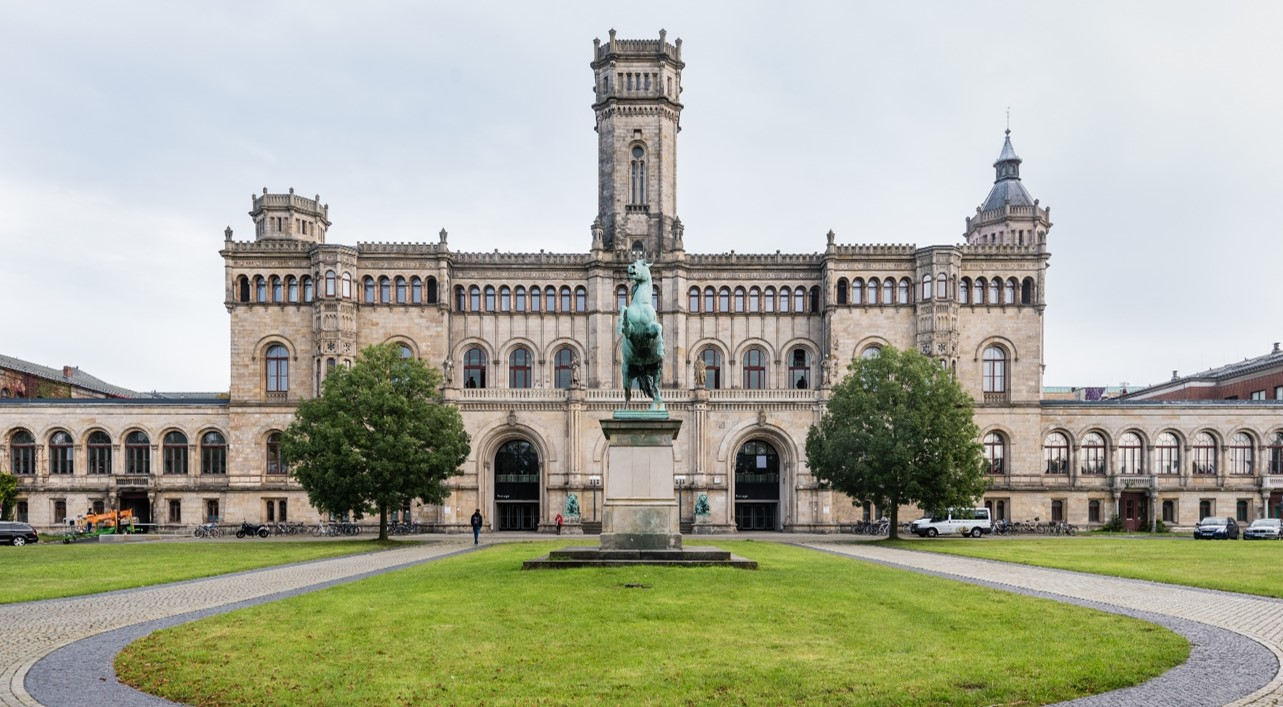
\includegraphics[width=0.65\textwidth]{figures/luh_default_presentation_title_image.jpg}}

% Title page: luhstyle
% \setbeamertemplate{title page}[luhstyle]
% % Add optional title image here
% \addtitlepageimage{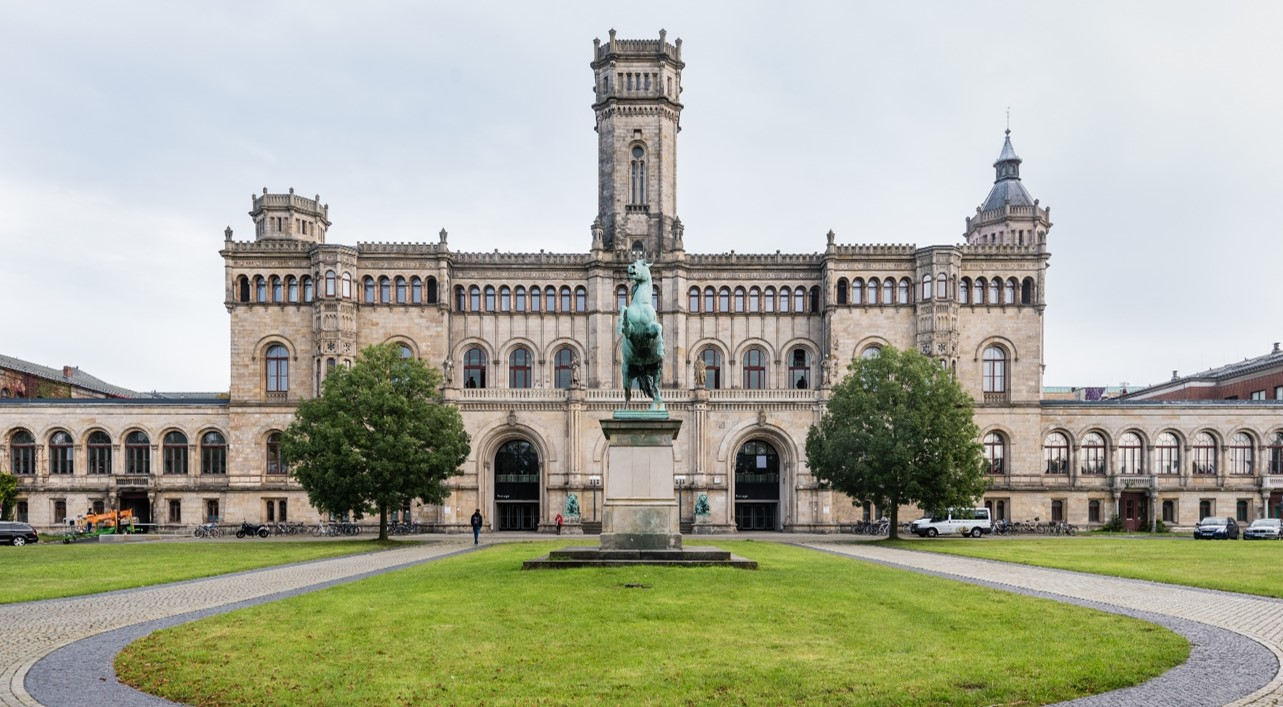
\includegraphics[width=0.75\textwidth]{figures/luh_default_presentation_title_image.jpg}}

\author[Lindauer \& Anand]{Marius Lindauer and Avishek Anand\\[1em]
	
\includegraphics[height=\logoheight]{../latex_main/figures/luh_logo_rgb_0_80_155.pdf}\qquad

\includegraphics[height=\logoheight]{../latex_main/figures/TNT_darkv4}\qquad

\includegraphics[height=\logoheight]{../latex_main/figures/L3S.jpg}	}
\date{Winter Term 2021
}


%%% Custom Packages
%----------------------------------------------------------------------
% Create dummy content
\usepackage{blindtext}

% Adds a frame with the current page layout. Just call \layout inside of a frame.
\usepackage{layout}


\title[Introduction]{iML: Shapley Values}
\subtitle{Discussion}

%\institute{}


\begin{document}
	
	\maketitle
	
\begin{frame}{Advantage: Fair Distribution and Solid Theory}
    
    \begin{itemize}
        \item the \emph{efficiency} property ensures that there is a fair distribution between the prediction and the average prediction 
        \item proven by the solid theoretical foundation of Shapley values 
        \begin{itemize}
            \item not given for most other methods discussed in this lecture series
        \end{itemize}
    \end{itemize}
    
\end{frame}

	
\begin{frame}{Disadvantage: Expensive}
    
    \begin{itemize}
        \item Computation of exact Shapley values is often infeasible (in high-dimensional spaces)
        \begin{itemize}
            \item $2^k$ possible feature subsets
            \item The contribution to each feature subsets needs further random samples
        \end{itemize}
        \pause
        \bigskip
        \item[$\leadsto$] Approximation of Shapley values via sampling
        \item However, number of samples required for a good approximation is unknown a priori
        \item Can still take quite some time and compute resources
    \end{itemize}
    
\end{frame}

\begin{frame}{Disadvantage: Interpretation}
    
    \begin{itemize}
        \item Shapley values are not really intuitive
        \item It's the contribution of a feature value to the difference between the actual prediction and the average prediction
        \item For people outside of ML (and economics), it might be hard to imaging all the possible feature subsets and we care about the contribution to these
    \end{itemize}
    
\end{frame}

\begin{frame}{Disadvantage: Dense}
    
    \begin{itemize}
        \item Each feature gets a Shapley value
        \begin{itemize}
            \item fairly unlikely that a reasonable feature gets $0$ as value
        \end{itemize}
        \item Humans often prefer sparse/selective explanations (especially in high-dimensional spaces)
    \end{itemize}
    
\end{frame}

\begin{frame}{Disadvantage: Hard to Act on It}
    
    \begin{itemize}
        \item Counterfactuals or LIME provide local explanations, which one can use to act on it\\ e.g., try to change features to obtain a more favorable outcome
        \item Shapley values "only" provide a single number per feature, but it does not tell you how to improve wrt these
        \begin{itemize}
            \item Even weights of a linear model provide more direction to act on it
        \end{itemize}
        
    \end{itemize}
    
\end{frame}

\begin{frame}{Disadvantage: Access to the True Data}
    
    \begin{itemize}
        \item Simply querying random feature vectors might lead to unreasonable feature importance
        \item We need access to samples from the true data distribution
        \begin{itemize}
            \item For example, the training data
        \end{itemize}
        \item Often not available, if we only want to examine a foreign model
    \end{itemize}
    
\end{frame}


\end{document}
